\chapter{Introduction}
Nous allons éclaircir dans ce chapitre la partie application du projet. \newline
Cette partie doit permettre de lire les valeurs envoyées par la STM32 via le port série, puis les afficher via une interface. \newline 
L'affichage doit être continu ainsi que la reception.

\begin{figure}[H]
	\centering
    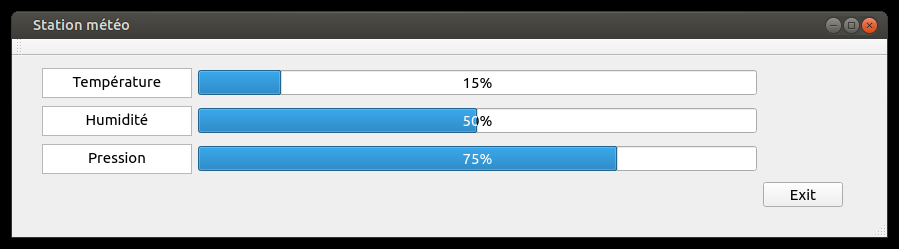
\includegraphics[width=\linewidth]{Figures/screen_app.png}
    \decoRule
    \caption[
    Aperçu de l'application]{
    Aperçu de l'application}
    \label{fig:Aperçu de l'application}
	\end{figure}
	
\section{Prise en main}

\begin{enumerate}
    \item Recupérer le projet 
        \begin{lstlisting}
            git clone https://github.com/ThomasAbg/StationMeteo
        \end{lstlisting}
    \item Executer le code:
        \begin{lstlisting}
            ./StationMeteo/InterfaceStation/Application_meteo
	    \end{lstlisting}
	    Il est aussi possible d'utiliser QtCreator.
	\item Optionnel, si vous souhaitez compiler le code: 
	    \begin{lstlisting}
        	votrechemin/StationMeteo/InterfaceStation/
        	Application_meteo.pro -spec linux-g++ 
        	CONFIG+=debug CONFIG+=qml_debug && 
        	/usr/bin/make qmake_all main.o
	    \end{lstlisting}
	    Il est aussi possible d'utiliser QtCreator.
\end{enumerate}	    



\chapter{Reception}

\section{Lecture données reçu}
Pour accédere aux données écrite dans le port série (dit "COM") il faut réquisitionner, le configurer.
\newline

\begin{figure}[H]
	\centering
    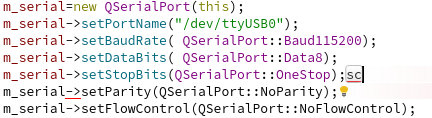
\includegraphics[width=0.7\linewidth]{Figures/config_comm.png}
    \decoRule
    \caption[
    Réquisition et configuration du port série]{
    Réquisition et configuration du port série}
    \label{fig:Réquisition et configuration du port série}
	\end{figure}

Maintenant viens le plus important, la lecture du port, pour celà je lie la fonction readyRead de la bibliothèque QSerialPort a ma fonction de lecture. La fonction readyRead renvoi toutes nouvelles données reçu dans le port qui à été configuré (objet: m_serial). 

\begin{figure}[H]
	\centering
    
\includegraphics[width=\linewidth]{Figures/lien_read.png}
    \decoRule
    \caption[
    Connecte la fonction readyRead fonction]{
    Connecte la fonction readyRead fonction}
    \label{fig:Connecte la fonction readyRead fonction}
	\end{figure}
	
\begin{figure}[H]
	\centering
    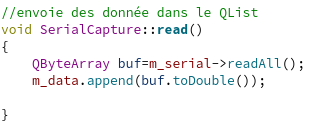
\includegraphics[width=0.5\linewidth]{Figures/read.png}
    \decoRule
    \caption[
    Fonction lecture données]{
    Fonction lecture données}
    \label{fig:Fonction lecture données}
	\end{figure}
	

\chapter{Multi taches}
Afin de pourvoir au besion d'afficher les données en même temps que l'on les recoivent, on est contraint à faire de faire deux action à la fois. \newline
Pour fairer celà il y a plusieurs solutions: multi-processus, multi-thread. \newline
J'ai choisie le multi-threading car les threads partagent les mêmes ressources (data) car ils se trouvent de le même processus, et ils sont plus légés que de réquisitionner un autre processus.

\begin{figure}[H]
	\centering
    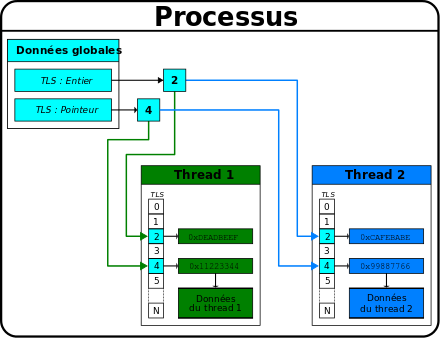
\includegraphics[width=0.5\linewidth]{Figures/illustration_threads.png}
    \decoRule
    \caption[
    Illustration threads]{
    Illustration threads}
    \label{fig:Illustration threads}
	\end{figure}

Dans notre cas le Thread1 est l'affichage et le Thread2 la lecture du port série.


\chapter{Affichage}

Pour faire l'interface de l'application j'ai utilisé le designer de Qt Creator, ce dernier donne acces à une large gamme de composants d'interface préconfigurés. 
Voici le résultat sur l'interface du designer.

\begin{figure}[H]
	\centering
    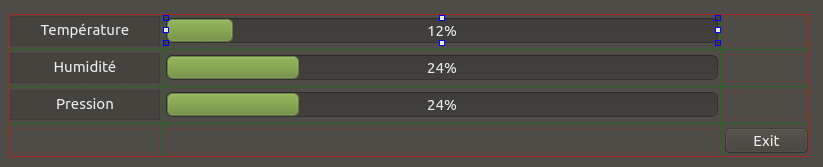
\includegraphics[width=0.8\linewidth]{Figures/ui-app.png}
    \decoRule
    \caption[
    Aperçu de l'application sur designer Qt Creator]{
    Aperçu de l'application sur designer Qt Creator}
    \label{fig:Aperçu de l'application sur designer Qt Creator}
	\end{figure}